% jbg: Questions we should answer in this question but which haven't been yet:
%
% - Can users choose not to answer a question?  If so, how is it
% scored?  If not, how are they prevented from skipping? 

% - Are there checks to ensure folks don't click randomly?  (I assume
% we're only using folks with good feedback, but often there are more
% checks built in to MT experiments ...  we don't right now (right?),
% although "reveal answer" might make people thing we do.)  

% - For the "answers don't bias" claim, do we have stronger data to back
% this up?

\section{Using human judgments to examine the topics}
\label{sec:tasks}
% Put little examples of tasks in figures; for word intrusion, put up an
% example of ``good'' topic and one example of ``bad'' topic to build
% intuition about why this task is meaningful.

% 1. The main goals of the tasks

Although there appears to be a longstanding assumption that the latent
space discovered by topic models is meaningful and useful, evaluating
such assumptions is difficult because discovering topics is an
unsupervised process.  There is no gold-standard list of topics to
compare against for every corpus.  Thus, evaluating the latent space
of topic models requires us to gather exogenous data.

In this section we propose two tasks that create a formal setting
where humans can evaluate the two components of the latent space of a
topic model.  The first component is the makeup of the topics.  We
develop a task to evaluate whether a topic has human-identifiable
semantic coherence.  This task is called \emph{word intrusion}, as
subjects must identify a spurious word inserted into a topic.  The
second task tests whether the association between a document and a
topic makes sense.  We call this task \emph{topic intrusion}, as the
subject must identify a topic that was not associated with the
document by the model.

% Our experiments are designed for people using Amazon's Mechanical
% Turk~\footnote{http://www.mturk.com} system, an online clearinghouse
% for tasks which require human-level intelligence such as developing
% gold-standard data for natural language processing~\cite{snow-08} or
% labeling images~\cite{imagenet-cvpr09}.  People use Mechanical Turk to
% perform short tasks for a small fee; we will use the term ``subjects''
% to refer to individuals who chose to complete our task.

% 2. Designed two tasks
\subsection{Word intrusion}
\label{sec:wordintrusion}
To measure the coherence of these topics, we develop the \emph{word
intrusion} task; this task involves evaluating the latent space
presented in Figure~\ref{fig:nyttopics:topic}.  In the word intrusion
task, the subject is presented with six randomly ordered words.  The
task of the user is to find the word which is out of place or does not
belong with the others, i.e., the \emph{intruder}.
Figure~\ref{fig:intruding_word} shows how this task is presented to
users.

\begin{figure*}[t]
\centering

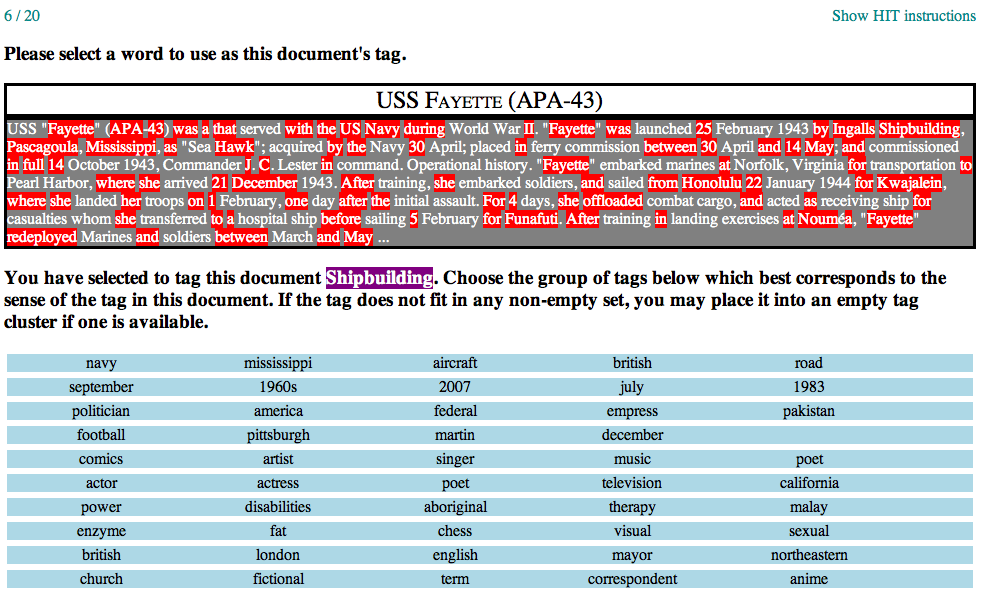
\includegraphics[width=0.90\textwidth]{figures/screenshots.png}

\caption{Screenshots of our two human tasks. In the word intrusion
  task (left), subjects are presented with a set of words and asked to
  select the word which does not belong with the others.  In the
  \emph{topic intrusion} task (right), users are given a document's
  title and the first few sentences of the document.  The users must
  select which of the four groups of words does not belong.}
\label{fig:intruding_word}
\end{figure*}

When the set of words minus the intruder makes sense together, then
the subject should easily identify the intruder.  For example, most
people readily identify \word{apple} as the intruding word in the set
\wordset{dog, cat, horse, apple, pig, cow} because the remaining
words, \wordset{dog, cat, horse, pig, cow} make sense together ---
they are all animals.  For the set \wordset{car, teacher, platypus,
  agile, blue, Zaire}, which lacks such coherence, identifying
the intruder is difficult.  People will typically choose an
intruder at random, implying a topic with poor coherence.

% sgerrish: I removed this paragraph, at least until we can measure this.
% The inter-subject agreement on the word intrusion task yields a
% measure of how semantically meaningful a set of words is: when all of
% the users agree on the intruder the set is semantically coherent; when
% none of them agree then the set is not.  

% jbg: I removed this footnote
% \footnote{The top words can be ranked either according to their
%   absolute probability mass in that topic, or according to their
%   probability mass in that topic relative to their unigram
%   probabilities.}

In order to construct a set to present to the subject, we first select
at random a topic from the model.  We then select the five most probable
words from that topic.  In addition to these words, an intruder word
is selected at random from a pool of words with low probability in the
current topic (to reduce the possibility that the intruder comes from
the same semantic group) but high probability in some other topic (to
ensure that the intruder is not rejected outright due solely to
rarity).  All six words are then shuffled and presented to the subject.

% In addition to being able to measure the semantic coherence of the
% topics using inter-subject agreement as described above, this task
% also enables the evaluation of whether the semantic divisions posited
% by a topic model correspond to those used by humans.  If the intruder
% as predicted by the topic model matched what the subjects thought was
% the intruder, then the topic found by the topic model resembles a set
% that our subjects believe is semantically coherent.

% While this
% approach also requires that models are able to select coherent topics,
% the first task provides an indication of whether the provided topics
% are reasonable.

For both the word intrusion and topic intrusion tasks, subjects were
instructed to focus on the meanings of words, not their syntactic
usage or orthography.  We also presented subjects with the option of
viewing the ``correct'' answer after they submitted their own
response, to make the tasks more engaging.  Here the ``correct''
answer was determined by the model which generated the data, presented
as if it were the response of another user.  At the same time,
subjects were encouraged to base their responses on their own
opinions, not to try to match other subjects' (the models')
selections.  In small experiments, we have found that this extra
information did not bias subjects' responses.

